\documentclass[12pt, a4paper]{report}

\usepackage[english]{babel}
\usepackage[utf8]{inputenc}
\renewcommand\familydefault{\sfdefault} % Sans Serif.

\usepackage[margin=2.54cm]{geometry}    % Page dimensions and margins.
\usepackage{graphicx}                   % Support the \includegraphics command and options.
\usepackage{float}

%%%
%%% Formatting sections and subsections.
%%%
\usepackage{textcase}
\usepackage[titletoc, title]{appendix}
\usepackage{titlesec}
\titleformat {\chapter}         {\large\bfseries\MakeUppercase}{\thechapter}{2ex}{}[\vspace*{-1.5cm}]
\titleformat*{\section}         {\large\bfseries}
\titleformat*{\subsection}      {\normalsize}
\titleformat*{\subsubsection}   {\normalsize}

\usepackage{chngcntr}
\counterwithout{figure}{chapter}    % No chapter number in figure labels.
\counterwithout{table}{chapter}     % No chapter number in table labels.
\counterwithout{equation}{chapter}  % No chapter number in equation labels.

\usepackage{booktabs}   % For much better looking tables.
\usepackage{url}        % Useful for inserting web links nicely.
\usepackage[bookmarks, unicode, hidelinks]{hyperref}

\usepackage{array}      % For better arrays (e.g. matrices) in math.
\usepackage{paralist}   % Very flexible & customisable lists (e.g. enumerate/itemize, etc.).
\usepackage{verbatim}   % Adds environment for commenting out blocks of text & for better verbatim.
\usepackage{subfig}     % Make it possible to include more than one captioned figure/table in a single float.
\usepackage{enumitem}
\setlist{noitemsep}


%%%
%%% Headers & Footers.
%%%
\usepackage{fancyhdr}
\pagestyle{empty}
\renewcommand{\headrulewidth}{0pt}
\renewcommand{\footrulewidth}{0pt}
\lhead{}\chead{}\rhead{}
\lfoot{}\cfoot{\thepage}\rfoot{}

\newcommand{\HeaderLineSpace}{-0.25cm}

\newcommand{\UniTextEN}{
UNIVERSITY POLITEHNICA OF BUCHAREST         \\[\HeaderLineSpace]
FACULTY OF AUTOMATIC CONTROL AND COMPUTERS  \\[\HeaderLineSpace]
COMPUTER SCIENCE AND ENGINEERING DEPARTMENT \\}
\newcommand{\DiplomaEN}{DIPLOMA PROJECT}
\newcommand{\AdvisorEN}{Thesis advisor:}
\newcommand{\BucEN}{BUCHAREST}

\newcommand{\UniTextRO}{
UNIVERSITATEA POLITEHNICA DIN BUCUREȘTI     \\[\HeaderLineSpace]
FACULTATEA DE AUTOMATICĂ ȘI CALCULATOARE    \\[\HeaderLineSpace]
DEPARTAMENTUL DE CALCULATOARE               \\}
\newcommand{\DiplomaRO}{PROIECT DE DIPLOMĂ}
\newcommand{\AdvisorRO}{Coordonator științific:}
\newcommand{\BucRO}{BUCUREȘTI}

\newcommand{\frontPage}[7]{
\begin{titlepage}
\begin{center}
{\Large #1} % Header (university, faculty, department).
\vspace{50pt}
\begin{tabular}{p{6cm}p{4cm}}

\includegraphics[scale=0.8]{pics/upb-logo.jpg} &
	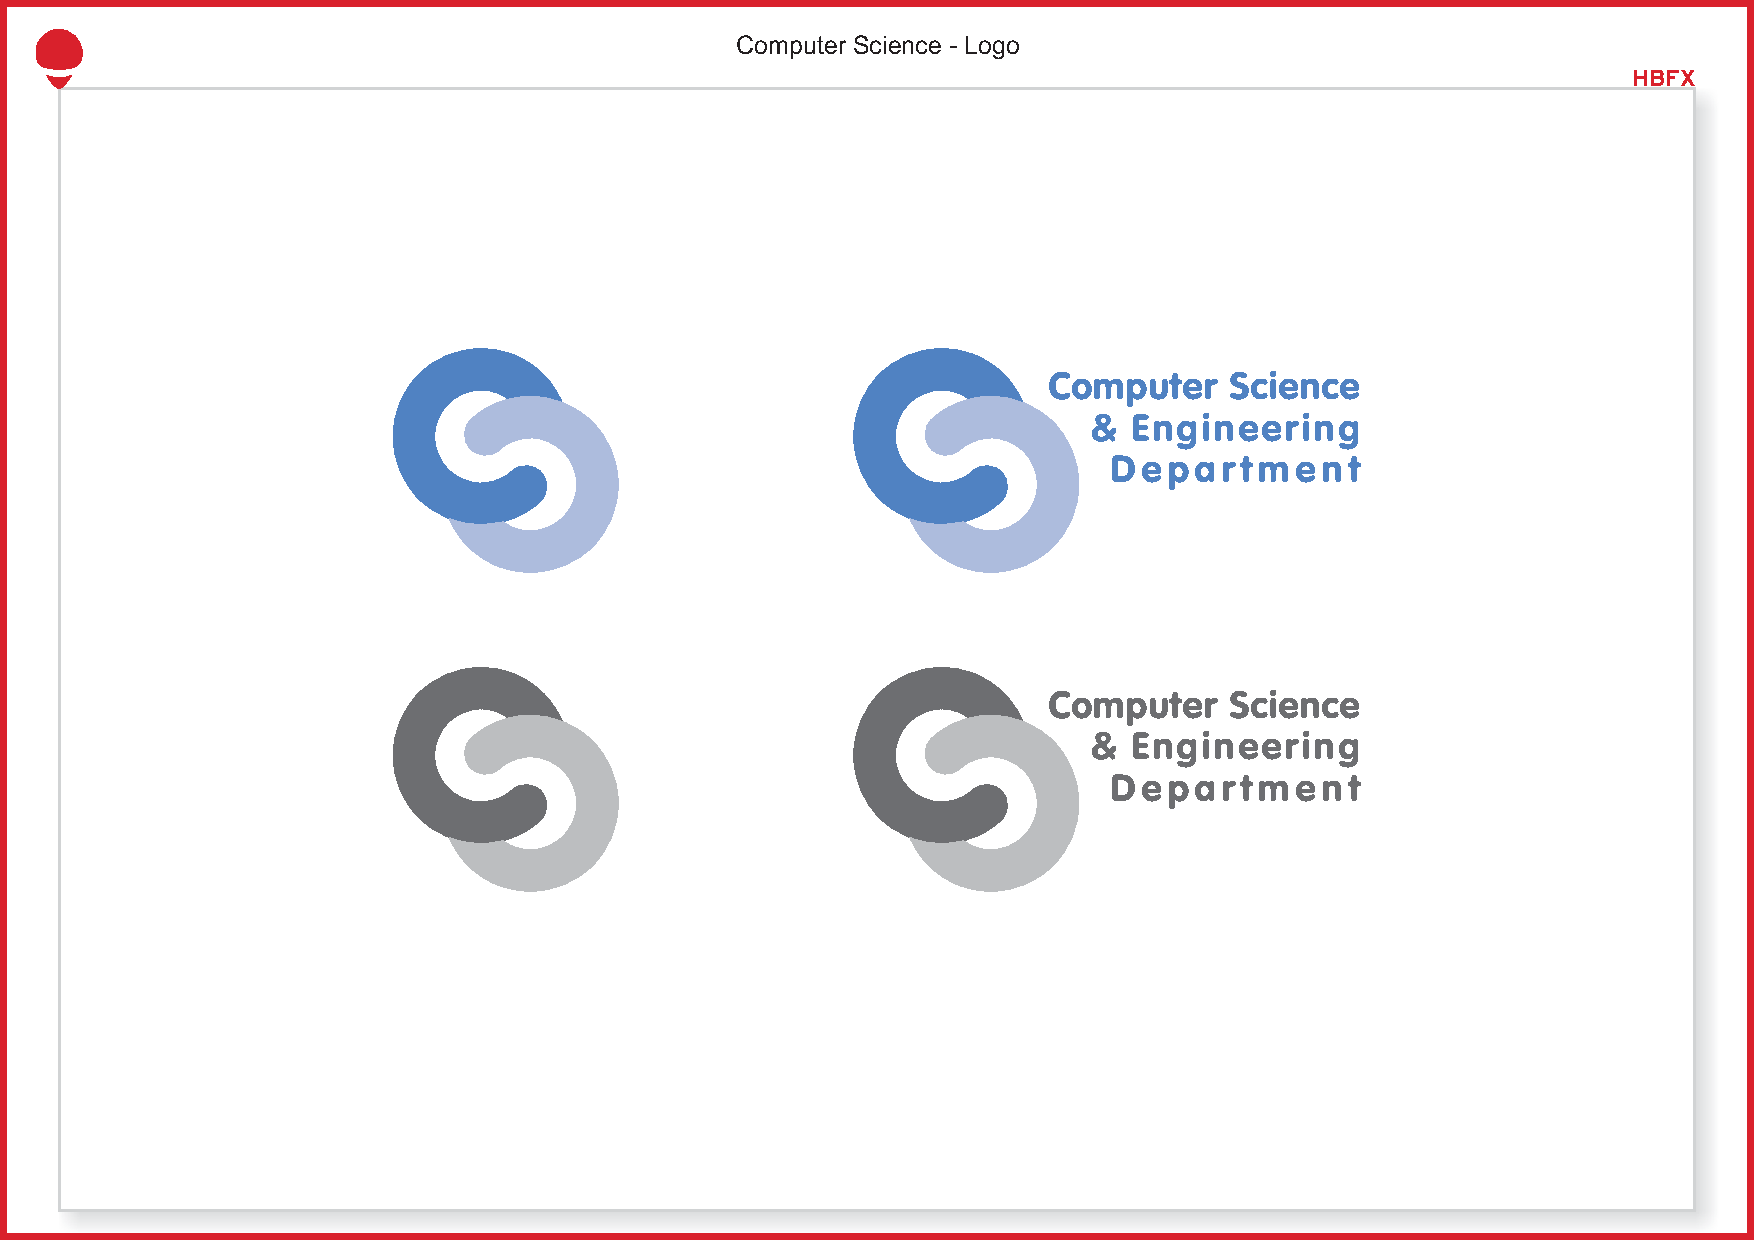
\includegraphics[scale=0.5,trim={14cm 11cm 2cm 5cm},clip=true]{pics/cs-logo.pdf}
\end{tabular}

\vspace{105pt}
{\Huge #2}\\                        % Diploma project text.
\vspace{40pt}
{\Large #3}\\ \vspace{0pt}          % Project title.
{\Large #4}\\                       % Project subtitle.
\vspace{40pt}
{\LARGE \Name}\\                    % Student name.
\end{center}
\vspace{60pt}
\begin{tabular*}{\textwidth}{@{\extracolsep{\fill}}p{6cm}r}
&{\large\textbf{#5}}\vspace{10pt}\\ % Scientific advisor.
&{\large{#6}        \vspace{10pt}}  % Advisor name.
\end{tabular*}
\vspace{20pt}
\begin{center}
{\large\textbf{#7}}\\               % Bucharest.
\vspace{0pt}
{\normalsize \Year}
\end{center}
\end{titlepage}
}

\newcommand{\frontPageEN}{\frontPage{\UniTextEN}{\DiplomaEN}{\ProjectTitleEN}{\ProjectSubtitleEN}{\AdvisorEN}{\AdvisorNameEN}{\BucEN}}
\newcommand{\frontPageRO}{\frontPage{\UniTextRO}{\DiplomaRO}{\ProjectTitleRO}{\ProjectSubtitleRO}{\AdvisorRO}{\AdvisorNameRO}{\BucRO}}

\linespread{1.15}
\setlength\parindent{0pt}
\setlength\parskip{8pt}


%%%
%%% Abstract macro.
%%%
\newcommand{\AbstractPage}{
\begin{titlepage}
\textbf{\large ABSTRACT}\par
\AbstractEN \vfill
\textbf{\large SINOPSIS}\par
\AbstractRO\par\vfill
\end{titlepage}
}


%%%
%%% Acknowledgments macro.
%%%
\newcommand{\AcknowledgmentsPage}{
\begin{titlepage}
\textbf{\large ACKNOWLEDGMENTS}\par
\Acknowledgments \vfill
\end{titlepage}
}


%%%
%%% Document settings.
%%%
\title{\ProjectTitleEN}
\author{\Name}
\date{\Year}


%%%
%%% Listing settings.
%%%
\usepackage{listings}
\usepackage{xcolor}

\definecolor{codegreen}{rgb}{0,0.6,0}
\definecolor{codegray}{rgb}{0.5,0.5,0.5}
\definecolor{codepurple}{rgb}{0.58,0,0.82}
\definecolor{backcolour}{rgb}{0.95,0.95,0.92}

\lstdefinestyle{mystyle}{
    backgroundcolor=\color{backcolour},
    commentstyle=\color{codegreen},
    keywordstyle=\color{magenta},
    numberstyle=\tiny\color{codegray},
    stringstyle=\color{codepurple},
    basicstyle=\ttfamily\footnotesize,
    breakatwhitespace=false,
    breaklines=true,
    captionpos=b,
    keepspaces=true,
    numbers=left,
    numbersep=5pt,
    showspaces=false,
    showstringspaces=false,
    showtabs=false,
    tabsize=2
}

\lstset{style=mystyle}

%%%
%%% End of template definitions.
%%% Title page.
%%%
\newcommand{\ProjectTitleEN}{Firecracker PCI Implementation}
\newcommand{\ProjectSubtitleEN}{Amazon.com, Inc.}
\newcommand{\ProjectTitleRO}{Implementarea PCI în proiectul Firecracker}
\newcommand{\ProjectSubtitleRO}{Amazon.com, Inc.}
\newcommand{\Name}{Andrei Răduță}
\newcommand{\AdvisorNameRO}{Conf.Dr.Ing. Răzvan Deaconescu}
\newcommand{\AdvisorNameEN}{Assoc.Prof. Răzvan Deaconescu}
\newcommand{\Year}{2020}

\newcommand{\AbstractEN}{
\begin{hyphenrules}{nohyphenation}
Firecracker has recently become a very popular and efficient open-source virtualization technology. The main purpose of this hypervisor is to run functions and containers in a safe and efficient manner. One of the Firecracker pillars is that it implements only the necessary components. The PCI (Peripheral Component Interconnect) bus is not among these capabilities. Yet, as this project develops, the need for this type of bus starts to arise.
\\The main problem is that it is impossible to connect a new device to a guest virtual machine while it is running. This diploma project adds within the Firecracker hypervisor a new way to administrate the emulated devices. This creates efficient management of the device model.
\\Among objectives is having a hot plugging functionality. A simple example is to increase the storage capacity of a running virtual machine by adding a new block device.
\\The solution consists of implementing a PCI bus within the Firecracker Virtual Machine Monitor. Each virtual machine will use an emulation of this hardware component.
\\The first result is increasing efficiency in working with external devices. The communication between the connected components is more coherent and well organized. Also, one can expect performance improvements due to better hardware resources usage and lower downtimes.
\end{hyphenrules}
}

\newcommand{\AbstractRO}{
\begin{hyphenrules}{nohyphenation}
Firecracker a devenit recent o tehnologie open-source de virtualizare foarte populară și eficientă. Scopul principal al acestui hipervizor este de a rula funcții și containere într-un mod sigur și eficient. Unul dintre pilonii proiectului Firecracker este că acesta conține doar componentele necesare. Magistrala PCI (Peripheral Component Interconnect) nu se numără printre aceste componente. Cu toate acestea, pe măsură ce acest proiect se dezvoltă, nevoia de acest tip de magistrală se simte mai puternic.
\\Principala problemă este că este imposibilă conectarea unui nou dispozitiv la o mașină virtuală în timp ce aceasta rulează. Acest proiect de diplomă adaugă la Firecracker o nouă modalitate de administrare a dispozitivelor externe, ce creează o gestionare eficientă a acestora.
\\Printre obiective se numără funcționalitatea hot plugging. Un exemplu simplu este acela de a crește capacitatea de stocare a unei mașini virtuale în timp ce aceasta rulează, prin configurarea și adăugarea unui nou dispozitiv bloc de date.
\\Soluția constă în implementarea unei magistrale PCI în cadrul proiectului Firecracker. Astfel, fiecare mașină virtuală va utiliza o emulare a acestei componente hardware.
\\Primul rezultat este creșterea eficienței în lucrul cu dispozitivele externe. Comunicarea dintre componentele conectate este mai coerentă și mai bine organizată. De asemenea, îmbunătățiri de performanță apar datorită unei mai bune utilizări a resurselor hardware, iar faptul că mașina virtuală suportă schimbări fără să fie oprită duce la perioade de indisponibilitate mai mici.
\end{hyphenrules}
}

\newcommand{\Acknowledgments}{
\begin{hyphenrules}{nohyphenation}
I have taken efforts in this project. Yet, it would not have been possible without the support and help of many individuals. I wish to extend my appreciation to everyone.
\\I would like to express my gratitude to Răzvan Deaconescu and Costin Carabaș. Their guidance, continuous feedback, and encouragement helped me in completion of this project.
\\I am very thankful to Dan Horobeanu and the Firecracker community. They were the source of the necessary information about this project. Also, their constant supervision aided me to choose the best and more efficient tools.
\end{hyphenrules}
}

\begin{document}

\frontPageEN
\frontPageRO

\AbstractPage

\AcknowledgmentsPage

\begingroup
\linespread{1}
\tableofcontents
\endgroup

%%%
%%% Text of the diploma project starts here.
%%%
\chapter{Introduction}\pagestyle{fancy}\label{introduction}

The purpose of a hypervisor is to create isolated environments which are virtual machines. Instead, the goal of an emulator is to reproduce in detail a hardware component and its behavior, so software fills in for hardware. This project involves emulating the PCI (Peripheral Component Interface) bus in such an isolated environment, created by Firecracker.

\section{Context}

The notion of external devices usually refers to peripherals that connect to a system. These may include network cards, sound cards, video cards. Also, within a system, there can exist block devices for storage, socket devices, serial console for communication, and so on. The role of a device model is to maintain the internal structures that reflect the state and the architecture of a system. This includes which devices and buses exist and how they connect.

What makes Firecracker so effective is that it performs only specific requirements very well. Thus, it implements a restricted model device that does not contain a PCI bus. But, both performance requirements and computing power increase, so new development demands appear. The goal for a virtual machine is to use the available resources with increased efficiency and also to have as few downtimes as possible. The PCI bus is a key component in ensuring these performances and also to broaden the perspective of new features.

\section{Problem}

The problem occurs from working with external emulated devices. Currently, in the Firecracker project, this process is not very efficient and scalable. The main drawback is that devices cannot connect to a guest virtual machine while it is running (at the post-boot time). Thus, one has to configure the connected devices before starting the guest (pre-boot time).

Yet, only the network and block devices (two of the five existing devices) can accept updates at the post-boot time. These patches include a step of notification to the Firecracker hypervisor and the virtual machine. As an example, changing the path or the size of the backing file of a block device is such an update.

Another problem arises from the use of hardware computing power. Thus, a virtual machine should use all the features that the underlying hardware has to offer. This is possible through a virtualization technique called hardware passthrough, which Firecracker does not support.

\section{Solution}

The solution consists of adding the PCI Express bus to the Firecracker project. Thus, each instance created by this Virtual Machine Monitor will contain an emulation of this bus.

The first reason why this decision is the right solution is that hot plugging is a native capability of PCI Express. Hot plugging is the ability of an operating system to recognize the changes in its device model while it is running. So, one can add or remove devices from a virtual machine at the pre-boot time. This creates much easier management of working with external devices.

The second reason is that the existence of a PCI bus makes the hardware passthrough mechanism possible. A real device can be directly connected to the emulated PCI bus within the guest virtual machine. So, the virtual machine can use all the computing power of a component as a GPU (Graphics Processing Unit). Given that the virtualization layer does not exist anymore, the obtained performance is almost native.

\section{Project Structure}

The \nameref{Motivation} chapter analyzes what problem solves this diploma project and what are the benefits of it. The base of this chapter consists of the requirements of the customers and the open-source community. There was also precise guidance from the advisers and mentors.

\nameref{State of the Art} presents the context of the current diploma project. It starts with general notions about what is virtualization and what is a bus. The next step presents PCI and PCI Express architecture and Firecracker environment. The current status section illustrates how all concepts combine and what shortcomings exist. To prove its relevance, the \nameref{Related Work} chapter presents benefits that the emulation of this bus brings in other hypervisors.

The \nameref{Use Cases} section gives more details about how this bus emulation will bring more advantages to the Firecracker project. One can notice that other usages may also exist.

This implementation has not something to compare with, because Firecracker is a very specific tool. Thus, the author decided to describe the development process to serve for other developers. The \nameref{Methodology} chapter contains details about which steps this work involved. One can consider this information when building a similar component.

\nameref{Solution Design} and \nameref{Implementation} expose the entire architecture and implementation of the solution. This section covers what the PCIe emulation looks like and how this component couples to the Firecracker device model. Aspects of the encountered problems are exposed.

The results and the implementation evaluation are presented in the \nameref{Evaluation} section.

The last chapter, \nameref{Conclusions and Further Work} presents the interpretation of this diploma project. It also introduces new ideas on how to continue this project. One should consider that this is part of a larger project and communicating with its community is a vital aspect.


\chapter{Motivation}\label{Motivation}

The current chapter presents the reasons to emulate the PCIe (PCI Express) bus in every guest virtual machine. This means implementing the bus in the Firecracker hypervisor.

The main motivation of the project is to ease the work with external devices for the Firecracker Virtual Machine Monitor users. The tree topology of the PCIe makes this bus an ideal solution to solve this problem. This is because a tree-shaped topology offers a very easy way to connect new devices by creating new branches. And this also makes the solution very scalable.

Nowadays, critical services receive increased attention. There are cases when updates or repairs need to take place without stopping or rebooting the guest virtual machine. Adding or removing devices from a system while it is running is a behavior named hot plugging. Hot plugging is a native capability of PCIe, along with an Advanced Error Reporting mechanism.

MSI (Message Signaled Interrupts) is another PCIe capability of interest for a system. An interrupt line is a hardware line over which devices can send signals to the CPU (Central Processing Unit), so it contains special out-of-band traffic. MSI is a solution to replace the traditional out-of-band interrupt lines with in-band messages. This means that the interrupt signals will circulate like normal messages. The key point is that these messages will have a special memory space where they are stored and from where the CPU will take them. This brings a series of improvements like less hardware needed and more controlled communication.

Having the PCIe device present brings the possibility of hardware passthrough. The guest will be able to use almost all the resources of the hardware device as if the virtualization layer does not exist. Figure~\ref{fig:gpu-passthrough} depicts a simple example. It shows a virtual machine that the host GPU (Graphics Processing Unit) as its own, so it will have near-native performance.

\begin{figure}[H]
\centering
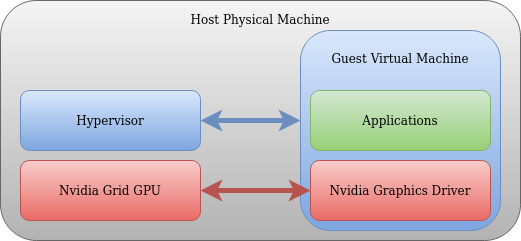
\includegraphics[height=5cm, keepaspectratio]{pics/gpu-passthrough.png}
  \caption{{GPU Pass-through}}
  \label{fig:gpu-passthrough}
\end{figure}

These are some of the reasons which confirm why this project has a big impact and drive it.


\chapter{State of the Art}\label{State of the Art}

This chapter presents several notions that this thesis discusses and works with. It details how virtual machines, hypervisors, devices, and PCI bus work and how all these intertwine.

Virtualization has emerged as a solution to the need to share the resources of a single server to many isolated operating systems. In the virtualization field, a hypervisor is a software, firmware, or hardware entity. It is also named VMM (Virtual Machine Monitor) and its roles are to create and run virtual machines. The name of the system on which the hypervisor runs is the host machine. A guest machine is a virtual machine created by the hypervisor.

A legacy virtual machine is a software entity that creates an environment where a unique guest operating system runs. So, on a physical server can run many virtual machines with various operating systems. In opposition, a container runs on top of a physical server and its host operating system. This makes containers look like lightweight virtual machines. So, using containers, on a single operating system instance can run many isolated workloads.

What is a bus is easy to understand making an analogy with a data highway. The bus makes connections between the main components categories inside a computer. These are the Central Processing Unit, Memory, and the Input/Output system. Each of these devices communicates on the bus, although each of them operates at very different speeds. Thereby, data, address, and control signals flow between CPU, memory, and peripherals on this pathway.

\section{PCI and PCI Express}

PCI (Peripheral Component Interface) bus appeared in the early 1990s. The people who developed it forms a group called PCISIG\footnotemark (PCI Special Interest Group). The role of this parallel bus is to provide a way to attach hardware devices (peripherals) to a computer.
\footnotetext{\url{https://pcisig.com}}

Figure~\ref{fig:pci-bus} shows an older system based on a PCI bus. Several devices share the PCI bus and are either connected directly to the bus or plugged into an intermediary connector. The North Bridge makes the connection between the high-speed components like the Processor and the PCI bus. A South Bridge connects PCI to the system peripherals, such as Ethernet ports.

An address space is the memory area that a program or a device can access. This memory is used for storing data or executing instructions and it can be physical or virtual. Thus, a device can have a specific range of the processor's address space. The access of the processor to the allocated address space is limited by the size of the bus and the number of registers.

\begin{figure}[H]
\centering
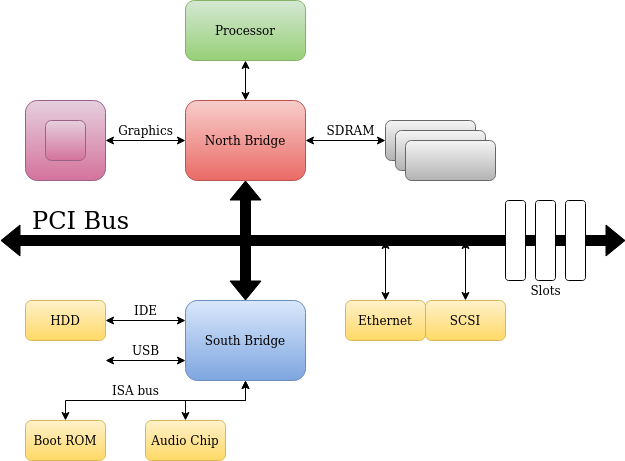
\includegraphics[width=\textwidth, keepaspectratio]{pics/pci-bus.png}
  \caption{PCI-based System}
  \label{fig:pci-bus}
\end{figure}

Peripheral devices have their own memory spaces which they use. Device drivers use this memory to control the devices and to pass information between them. Shared memory between the processor and the devices will make the communication possible between them\footnotemark. PCI architecture supports three address spaces as shown in figure~\ref{fig:pci-address-space-mapping}: I/O (Input/Output) address space, memory address space, and configuration address space.
\footnotetext{\url{http://www.science.unitn.it/~fiorella/guidelinux/tlk/node66.html}}

The method for accessing each of these address spaces depends on the system the PCI bus is connected to. On x86 systems, the CPU accesses memory spaces using the \texttt{in} and \texttt{out} instructions. Each function of a PCI device contains up to six BARs (Base Address Registers). A BAR specifies how much memory a PCI function needs and after PCI device enumeration it holds the base address of the allocated memory block. So, the CPU can interact with a PCI function by reading or writing to its I/O space or MMIO (Memory-Mapped I/O) space indicated by a BAR.

The configuration space represents the internal registers of a PCI function and it has 256 bytes. To access it, one has to access the Address and Data PCI I/O ports (a port is a memory address). \texttt{CF8h-CFBh} port sets the PCI configuration space address register and from \texttt{CFCh-CFFh} port the user reads or writes data. On any recent system, MMIO is also a solution to access the configuration space of a PCI function.

\begin{figure}[H]
\centering
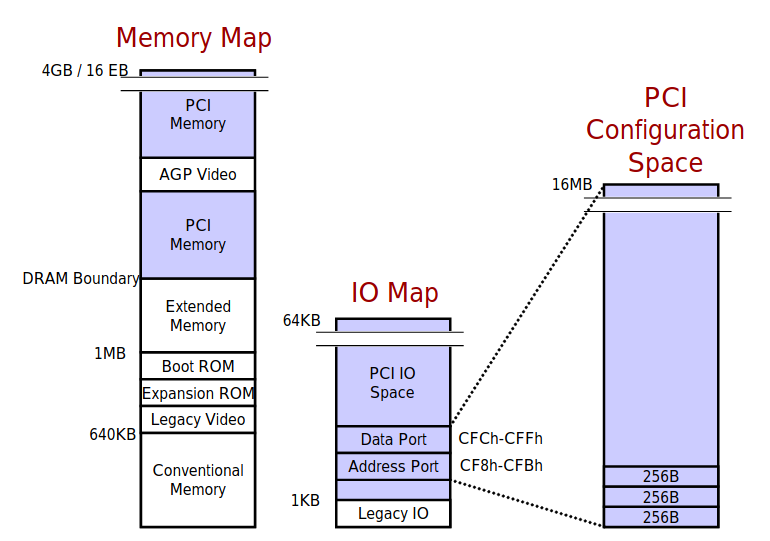
\includegraphics[width=\textwidth, keepaspectratio]{pics/pci-address-space-mapping.png}
  \caption{{PCI Address Space Mapping (Jackson, 2012, p.26)}\cite{book_pci_express}}
  \label{fig:pci-address-space-mapping}
\end{figure}

PCI Express is a high-speed serial bus, designed to replace the older PCI. Some of the improvements are higher system bus throughput and better performance scaling for bus devices. The throughput term refers to how much data can be transferred from source to destination within a given time frame. Instead of one bus that handles data from many sources, PCIe has a central node that controls several point-to-point connections. It introduces a more detailed error detection and reporting mechanism named Advanced Error Reporting.

Yet, one of the most relevant functionality for the current thesis is the native hot plug capability of PCIe. Hot swapping is the replacement or addition of components to a computer system while it is running. Hot plugging refers to the addition of components only. This mechanism utility consists of making changes to a system without interrupting it. So, one can add or replace faulty components or peripherals without stopping the main services.

Figure~\ref{fig:pcie-topology} illustrates a simple PCI Express topology which is not a complex scheme, as one can see. It is similar to a tree-topology that does not contain loops (closed circuits) and has the root in the Root Complex node. This type of topology is a good design decision for systems that have to adapt to increasing performance demands. This is because a new leaf or new branch can be added very easily. A leaf consists of a PCIe endpoint or a Legacy (PCI) endpoint. A switch or a bridge can create a new branch to which other nodes will connect. A switch is a component that forwards traffic between nodes, and a bridge connects two buses.

The most important component between the CPU and the PCIe bus is the Root Complex. This node connects to the processor and the main memory through various interfaces. It also contains the Host Bridge, which is the device that acts on the behalf of the CPU to communicate with the rest of the system. So, every device connects by a separate serial link to the Root Complex. Within a serial transmission, each bit of data is sent sequentially along the communication channel, and it is much faster than parallel transmission.

\begin{figure}[H]
\centering
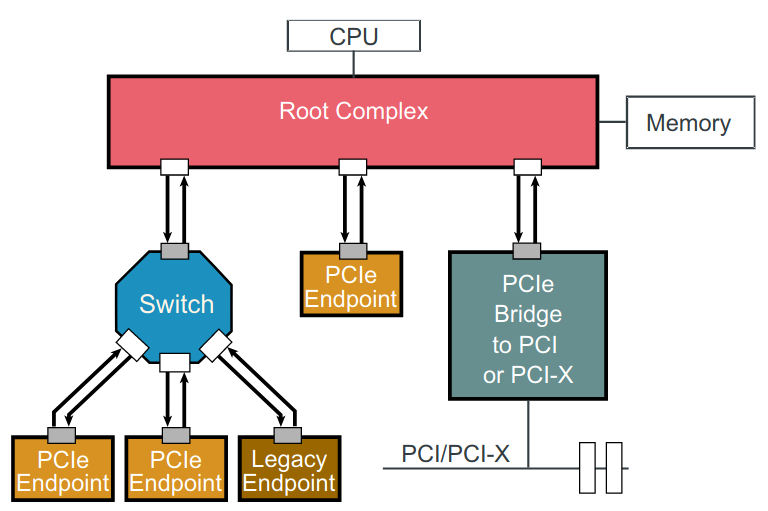
\includegraphics[width=\textwidth, keepaspectratio]{pics/pcie-topology.png}
  \caption{{Example of PCIe Topology (Jackson, 2012, p.47)}\cite{book_pci_express}}
  \label{fig:pcie-topology}
\end{figure}

PCI Express is a layered protocol, consisting of a transaction layer, a data link layer, and a physical layer. The communication between the topology nodes works based on well-defined packets. The transaction layer takes care of encapsulating and de-encapsulating data from devices in TLPs (Transaction Layer Packets). A TLP is composed of header, data, and digest.

\section{Firecracker Environment}

{Firecracker}\cite{firecracker_website} is a great innovation in the field of hypervisors and server-less computing. Its purpose is to create and manage secure, multi-tenant containers, and function-based services. Server-less allows one to build and run applications and services without thinking about servers. What makes Firecracker special is its way of combining the notions of virtual machines and containers. So, this hypervisor puts together complexity, security, isolation, fast startup, and high density. Because of it, the virtual machines created by Firecracker are named microVMs.

Among the main pillars of the Firecracker is that it contains only the essential and needed components. This improves security and efficiency but can impose other drawbacks. One of these drawbacks is that new complex functionality is hard to add, due to the lack of various components. Currently, the only available emulated devices are:
\begin{itemize}
    \item virtio-net - networking device.
    \item virtio-block - block I/O device.
    \item virtio-vsock - host/guest communication device.
    \item serial console.
    \item minimal keyboard controller - used only to stop the microVM.
\end{itemize}

To manage and interact with its emulated devices, Firecracker has two device managers. The purpose of each device manager is to access one of the types of memory space mentioned above. So, they are a PIO (Port-based I/O) device manager and an MMIO (Memory Mapped-based I/O) device manager. Firecracker has internal structures for representing the memory and the interactions with it. The details of interest for this project are how the PIO device manager works because it will ensure communication with the PCI Host Bridge.

Figure~\ref{fig:firecracker-architecture} depicts the Firecracker architecture. It is written in Rust and one can observe that the host functionality depends on two Linux Kernel facilities. These two virtualization capabilities are the KVM\footnote{\url{https://www.linux-kvm.org}} (Kernel-based Virtual Machine) module and the VirtIO\footnote{\url{https://developer.ibm.com/technologies/linux/articles/l-virtio}} Framework. A program called \textit{jailer} improves security, by creating a second line of defense, after virtualization. So, each microVM has an extra isolation layer using common Linux user-space security barriers.

The communication between the host and the guest machine uses a RESTful API\footnotemark. Customers can use the API for common actions such as starting or stopping the virtual machine. It is also useful for configuring properties of the microVM, including the connected devices. Even if the requests offered by this API can be sent anytime, some of them will be successful only when the virtual machine is not running.
\footnotetext{\url{https://github.com/firecracker-microvm/firecracker/blob/master/docs/api_requests}}

Firecracker acts as a next-generation hypervisor for server-less workloads (functions and containers). The minimal design of its device model does not support the most legacy devices or hardware pass-through. But new use cases and needs appear with the advance of the hardware computing power and the software demands. Thus, the major goal is that the virtualization software can maximize the use of all available resources.

The {publication}\cite{firecracker_article} of the Amazon Science team illustrates more details about the purpose and architecture of Firecracker. It provides insight into what replacements and improvements over the traditional virtualization techniques are. The traditional view is that there is a choice between virtualization and container technologies.

\begin{figure}[H]
\centering
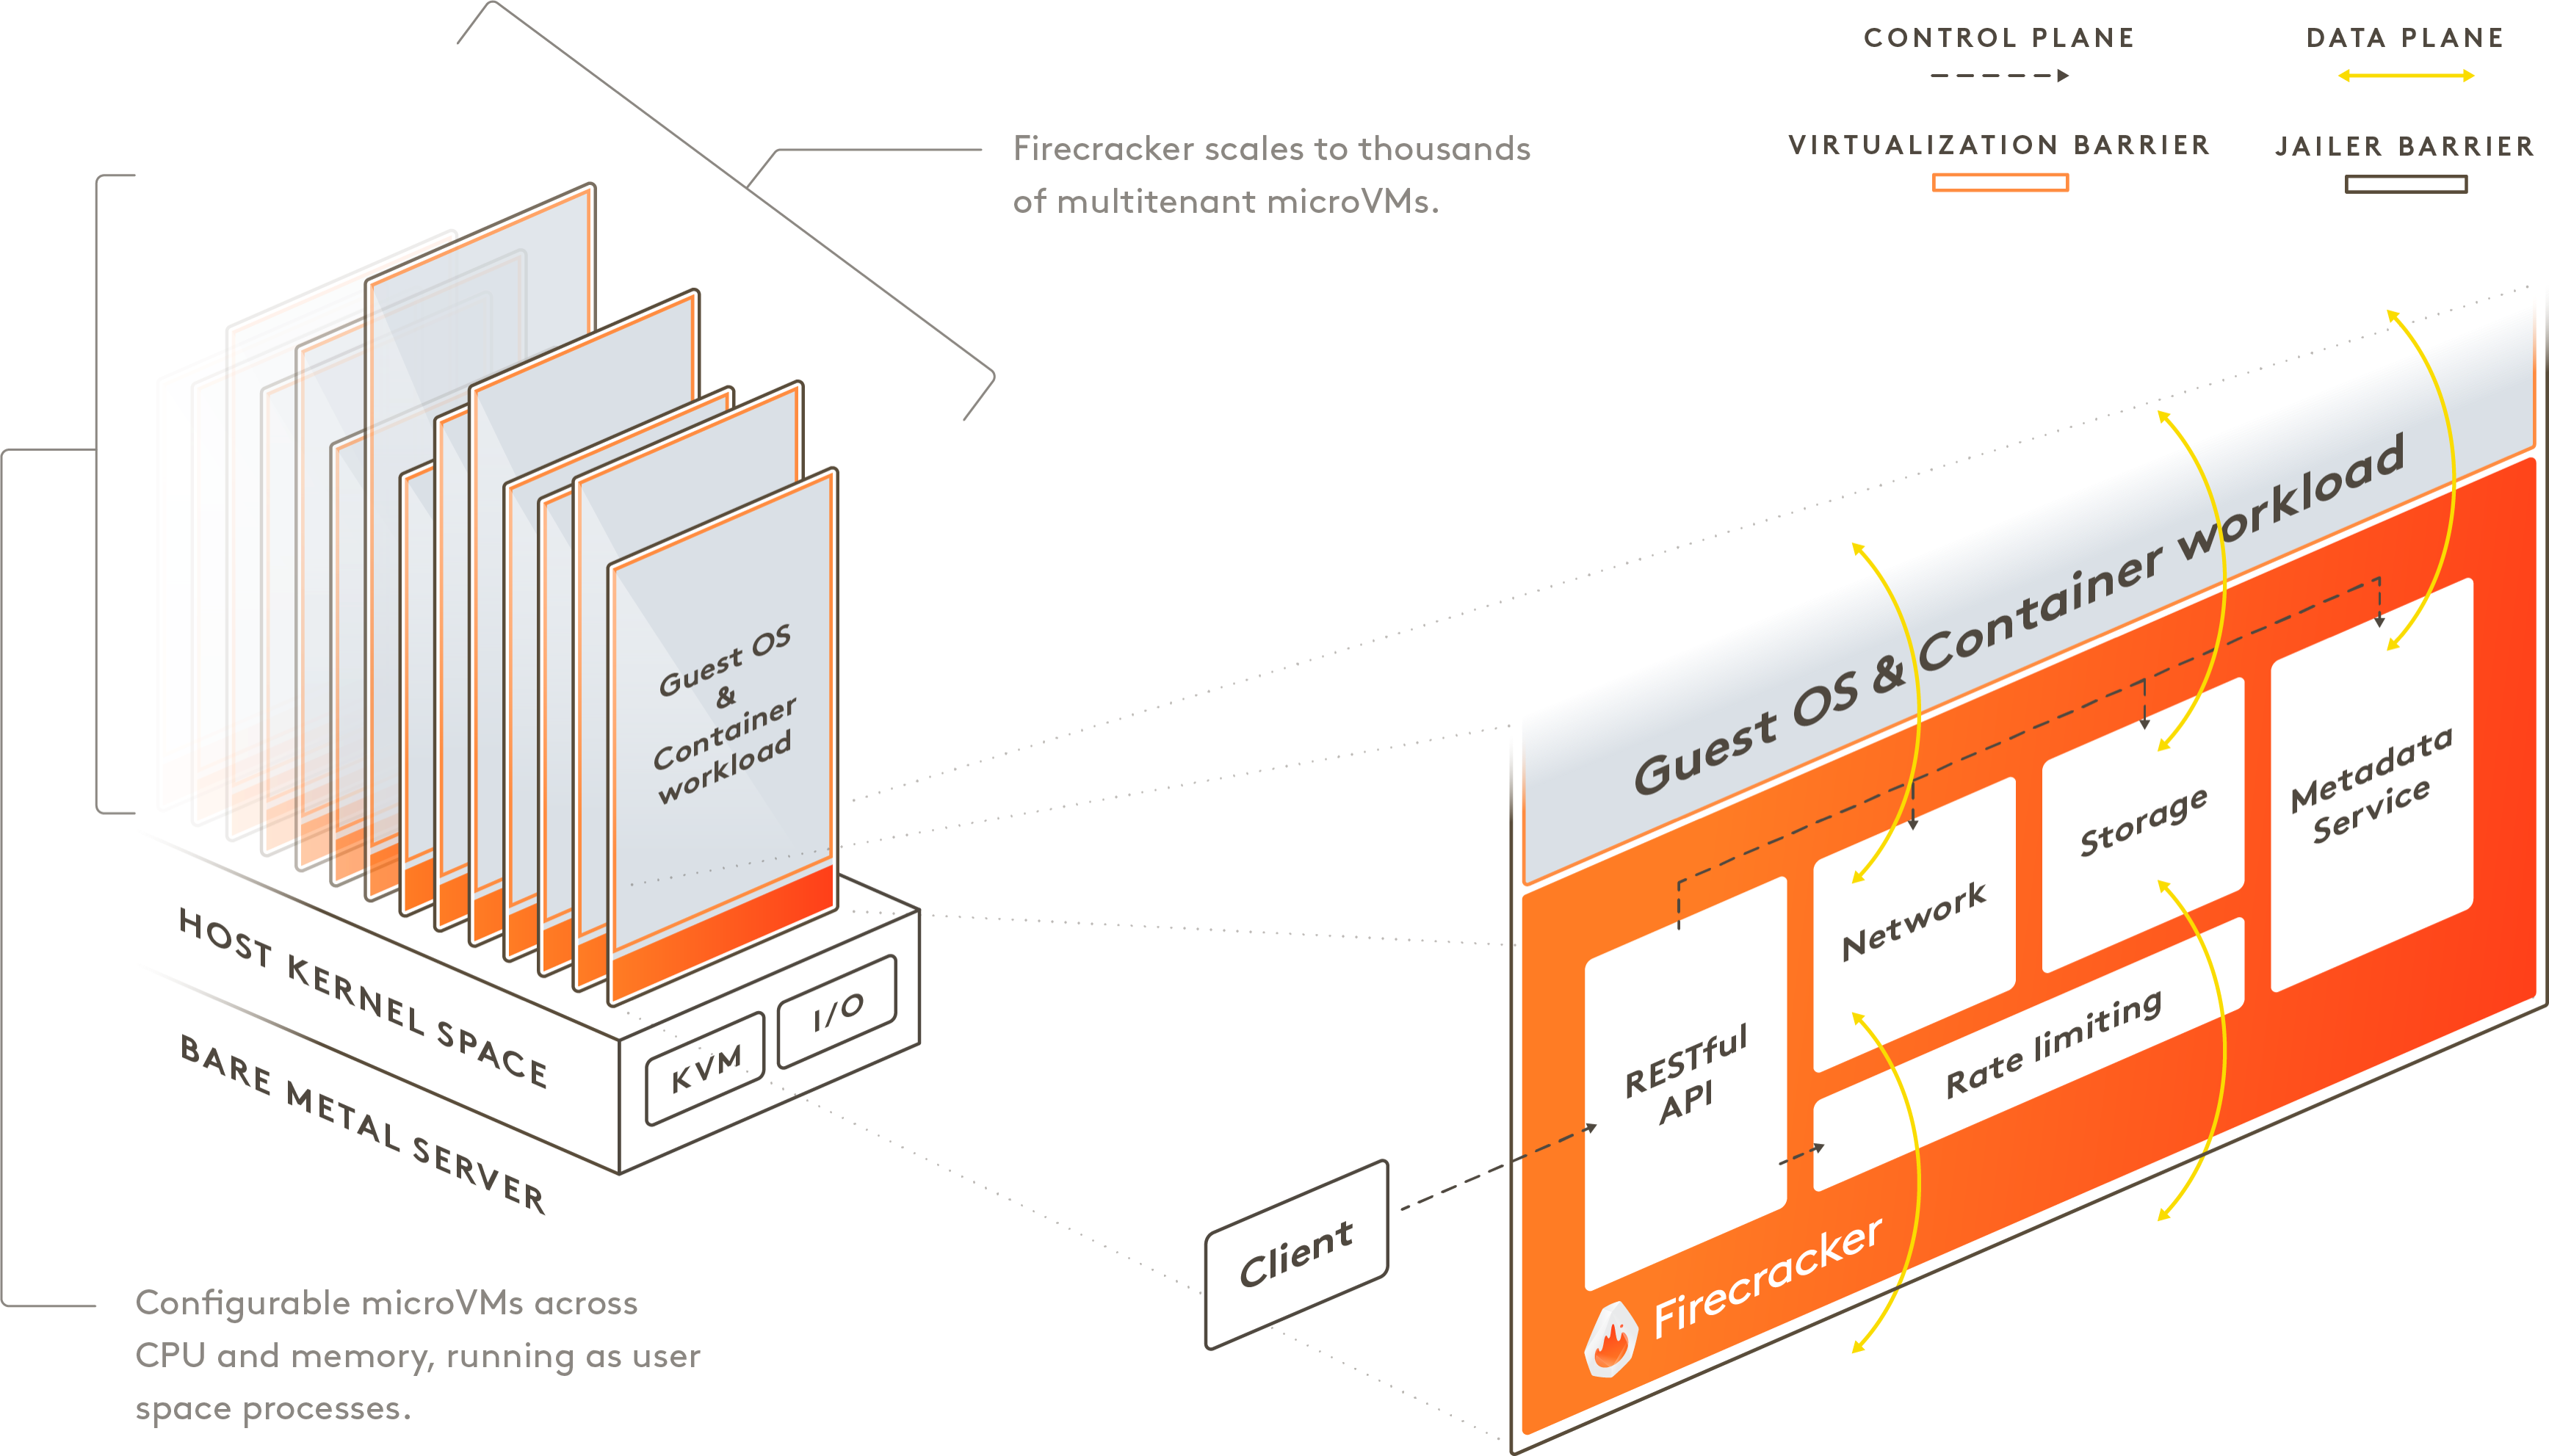
\includegraphics[width=\textwidth, keepaspectratio]{pics/firecracker-architecture.png}
  \caption{{Firecracker architecture}\cite{firecracker_website}}
  \label{fig:firecracker-architecture}
\end{figure}

\section{Current Status}

As one can see, a complex bus like PCI Express is not found in the Firecracker hypervisor. Firecracker has not an implementation of this type of bus because there was not a great need for it for the given requirements. But as this project develops, the need for better and scalable management of the external devices arises.

There are two methods to connect a device to a virtual machine created by Firecracker. The first one is by specifying it in a configuration JSON file, which the microVM will use to boot. The other one is by using the RESTful API requests to make these configurations.

The important detail in the case of both methods is the configuration moment. Any update to the configuration takes effect only before the guest starts, so at the pre-boot time. At the post-boot time, there exists only the possibility to update (not to add) a network device or a block device. But besides the operations of the update, there is an extra step by which Firecracker and the virtual machine are notified using a PATCH request.

Thereby, managing devices that interact with the virtual machine is difficult. The whole process is cumbersome, prone to human errors, and most important, it is not flexible. Adding or removing devices implies restarting the microVM. Also, updating a device configuration needs extra steps to notify the guest machine and the hypervisor. These things can cause great losses of time and operating problems. Moreover, with the implementation of a PCI bus, advanced architecture improvements become available. Next, examples from other virtualization projects present how these theoretical notions look in practice.


\chapter{Related Work}\label{Related Work}

This chapter presents other existing hypervisors, to create a more clear idea to the reader where Firecracker locates. In these examples, the PCI bus is already implemented and it brings some of the benefits mentioned above. Of course, a punctual comparison cannot be made, because the usages of each project are quite different.

\section{QEMU}

QEMU\footnotemark (Quick Emulator) is an open-source emulator that performs hardware virtualization. It provides a set of different hardware and device models for the machine, enabling it to run a variety of guest operating systems. Thus, it translates instructions from one architecture to another and makes it possible to run applications on unsupported architectures.
\footnotetext{\url{https://www.qemu.org}}

Comparing the number of lines of code, Firecracker represents approximately 4\% of the size of the QEMU project. Thus, QEMU, which is written in C, is a much more complex project, which can emulate various operating and devices. This project is used by a wide range of clients and due to it is complex, the level of security is lower than that of Firecracker.

QEMU contains implementations for both PCI and PCIe. One of the most important use cases is the role of the PCI bus in device passthrough. Thus, the guest virtual machine can directly use the underlying hardware of the host to its greatest capacity. A good example of this topic is the passthrough of a graphics card. Providing native graphics performance to the virtual machine is useful for computational-intensive activities.

\section{Cloud Hypervisor}

Cloud Hypervisor\footnotemark is an open-source Virtual Machine Monitor focused on running cloud workloads. A cloud workload is the amount of work that one would like to run in the Cloud. This hypervisor is also written in Rust and some features are common between it and Firecracker.
\footnotetext{\url{https://github.com/cloud-hypervisor/cloud-hypervisor}}

A running guest started by Cloud Hypervisor supports hot plugging, based on the PCI transport. The following devices are supported: virtio-block, virtio-net, virtio-pmem (persistent memory), virtio-fs (file system), and virtio-vsock. It also supports the change of a PCI Base Address Register (the base memory address of a device) without interrupting the guest.


\chapter{Use Cases}\label{Use Cases}

The current chapter will present the use cases where the work of this diploma project is useful.

In the 2020 Research Road map of the Firecracker project, the first request is machine learning acceleration\footnotemark. Thus, doing hardware-accelerated inferences in a server-less environment is a compelling use case. For this to be possible, emulating a PCI bus is a key step, because the host GPU can be connected to the emulated bus. GPUs are popular for AI (Artificial Intelligence) work. They continue to evolve in a direction to ease deep learning, both for training and inference in devices such as self-driving cars. This publication\cite{gpu_passthrough} makes some measurements on the GPU passthrough performance using different hypervisors. Developing a PCI bus will further allow the device passthrough, which is a more general use case.
\footnotetext{\url{https://github.com/firecracker-microvm/firecracker/issues/1179}}

The WeaveWorks Ignite\footnotemark community showed interest in the subject, during the writing of this diploma project. This demonstrates once again the real utility that this work brings. Further, the facilities and the help offered by the open-source community is a strong confirmation.
\footnotetext{\url{https://github.com/weaveworks/ignite}}

No downtime is a very important affirmation for the users of the production environment. This capability makes it possible for an administrator to manage systems without shutting them down. PCIe offers this behavior of hot plugging. In this {study}\cite{firecracker_study} about Firecracker, the need for hot plugging is reinforced, to avoid interventions to the workload. This facilitates to add, for example, more storage as a new block device or more bandwidth as a new network device. Whenever a virtual machine needs more resources, it does have to reboot for the effect to take place. In consequence, critical services do not have to stop.

The Firecracker development team has found the optimal middle ground between virtualization and containers. Two public available server-less computer services at Amazon Web Services use it: Lambda\footnote{\url{https://aws.amazon.com/lambda}} and Fargate\footnote{\url{https://aws.amazon.com/fargate}}. Firecracker supports millions of production workloads and trillions of requests per month from hundreds of thousands of customers\footnotemark.
\footnotetext{\url{https://aws.amazon.com/blogs/opensource/recap-part-three-open-source-reinvent-2019}}

The two use cases already mentioned would bring even greater demand and use from customers. Device passthrough need comes from fields such as Artificial Intelligence and Machine Learning. Having hot plug capabilities would make Firecracker a very useful tool in systems administration. Thus, it can manage systems that contain critical services that cannot be stopped when updates are made. Taking advantage of its efficiency and scalability, this hypervisor can bring a huge impact on many other projects.


\chapter{Methodology}\label{Methodology}

This chapter serves as a set of instructions. It can be useful when a new component is added to the Firecracker project or to better understand and continue the current work.

Before I started this diploma project, my knowledge of PCI architecture was general and I had not read or written any line of Rust code. So, the first step was to do more detailed research on both topics. Thus, I read \textit{PCI Express Technology}\cite{book_pci_express} to deepen how PCI and PCI Express work and \textit{The Rust Programming Language}\cite{book_rust_programming} to understand how to best use Rust.

The second step was to explore Firecracker to better understand how it operates. I read all the documentation provided on its website, plus other articles and videos found on the Internet about this hypervisor. Last but not least, I adopted a method of learning by doing. I made my own copy of the repository and I built the binary from it. Finally, I managed to run myself an Alpine Linux instance using Firecracker, from a custom kernel image and rootfs.

Although I had mentors from both University Politehnica of Bucharest\footnote{\url{https://upb.ro/en/faculties/the-faculty-of-automatic-control-and-computer-science}} and
Amazon.com, Inc.\footnote{\url{http://romania.amazon.com}}, my questions were not only addressed to them. Since Firecracker is an open-source project I announced my intention to put in place the PCI bus. So, I started to ask beginner questions for a better understanding of the project. This allowed me to figure out how can to use the existing code in an efficient manner. It also showed me how welcoming and responsive the open-source community is.

Next, I began to read the implementation of the PCI bus from other projects. There is a complex implementation within QEMU written in the C language, from which I understood some general aspects. Furthermore, Cloud Hypervisor has been more helpful because it has common roots with Firecracker. Also, it is written in Rust, so I could learn this programming language faster. The problem with this aspect was the fact that it is difficult to make analogies between these projects. The reason is that they have quite different components and purposes.

The next steps were to write code and to build the new library. It was a back-and-forth process between the theoretical part and the practical part. I added pieces of code (with unit tests) until I achieved the desired functionality. I am an autonomous and self-driven engineer, but in the moments when I got stuck, I received help from my mentors or the community.

In the end, I can't say how important reliable documentation of the code is. Its main focuses are development, maintenance, and knowledge transfer to other developers. I had big troubles understanding code that was summary or not documented at all. So, for each written code block, I made sure to add concise and explicit documentation.


\chapter{Solution Design}\label{Solution Design}

This chapter explains how the solution architecture looks like. Figure~\ref{fig:firecracker-device-model} illustrates the current Firecracker device model. Based on how the CPU communicates with the memory of the emulated devices, this model involves two device managers. The red-marked component is the root of a PCI Express topology and is where PCI bus merges with Firecracker.

\begin{figure}[H]
\centering
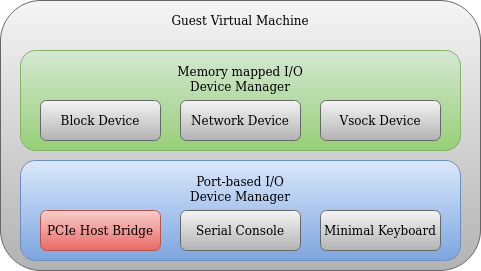
\includegraphics[height=8cm, keepaspectratio]{pics/firecracker-device-model.png}
  \caption{{Firecracker Device Model}}
  \label{fig:firecracker-device-model}
\end{figure}

The first manager administrates devices that use an MMIO mechanism. MMIO uses the same address space to address both memory and I/O devices. The memory and registers of the I/O devices are mapped to (associated with) address values. So when an address is accessed by the CPU, it may refer to a part of physical RAM, or it can instead refer to memory of a device. Thus, an instruction that would access the memory address space can access the I/O address space too. Specialized hardware takes care of fulfilling this mapping.

The second manager operates the PIO devices. This mechanism uses a special class of CPU instructions designed for accessing I/O address space. I/O devices have separate address space from general memory, thing which is accomplished by the hardware. PIO can use the same address bus to access the memory but operate all the available devices with only a few hardware lines. This is important because it avoids the under-utilization of system resources.

The communication with the PCI device is like communication with a serial console.  When a read or write is made to a particular I/O port (address), an entity that manages that I/O port receives a notification as an interrupt. Thus, values from registers and memory will help to interpret what was the operation and what is its result. The locations for the serial console ports\footnotemark can vary, but in most cases, the first two COM ports will be at \texttt{3F8h} and \texttt{2F8h}.
\footnotetext{\url{https://wiki.osdev.org/Serial_Ports}}

As shown in figure~\ref{fig:pci-address-space-mapping}, PCI communication uses two 32-bit I/O ports. The first address is at \texttt{CF8h}. This register specifies the configuration address of the access on the bus (where will be the access). The second address is at \texttt{CFCh} and accessing it will generate the actual configuration access. Then, depending on the type of the operation, the PCI device reads from or writes data to this register. The drivers of the devices within the operating system take care of observing the generation of these accesses. Also, the drivers decide how to interpret the information and how to process it.

The solution to the mentioned problems and motivations mentioned in the previous chapter takes the form of a new I/O device. It connects to the PIO manager along with the serial console and the minimal keyboard. The work done by the new device is to respond to read and write operations in the space dedicated to the PCI bus. Further, it depends on the internal logic of the PCIe topology how these operations get to the connected devices.

The name of the new component is Host Bridge and it is part of the Root Complex as presented in figure~\ref{fig:pcie-root-complex}. It will act on behalf of the CPU to interact with the devices connected to the system through PCI. Thereby, the specific role of this entity is to translate all the requests from the CPU in PCIe messages and the other way around.

\begin{figure}[H]
\centering
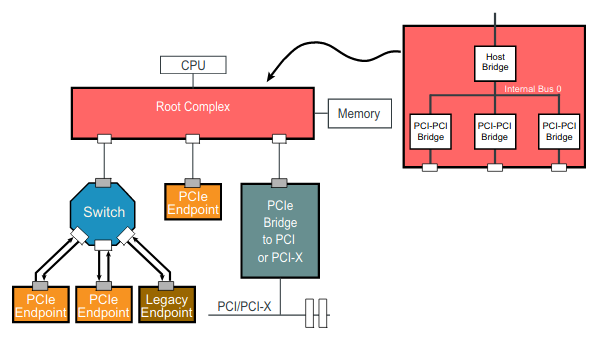
\includegraphics[height=8cm, keepaspectratio]{pics/pcie-root-complex.png}
  \caption{{PCIe Root Complex Structure (Jackson, 2012, p.51)}\cite{book_pci_express}}
  \label{fig:pcie-root-complex}
\end{figure}

The initial design of the Host Bridge device is like the Serial Console implementation. So, the first need is to have a device that will respond to the requests made to the PCI I/O ports. The PCI Express book\cite{book_pci_express} brings the theoretical elements about how the PCIe devices should look and communicate (the protocol). PCIe specification permits a system to have up to 256 buses. Each bus can have up to 32 devices and each device can have up to 8 functions. A key point in the solution design is a 16-bit number that locates a device's function. Its abbreviation is BDF (or B/D/F) and it stands for Bus, Device, Function. This number helps to identify where a device exists in the PCIe tree-topology. Based on this, each communication channel can use a serial point-to-point model.

The solution also takes into account existing implementations to complete the theoretical background. The Cloud Hypervisor project, which is under the same license as Firecracker, is a reference point. Although they are different projects, the implementation of the PCI bus from Cloud Hypervisor has given some ideas and clues.

The next step in the design of the solution was to achieve successful communication between the operating system and Host Bridge. Depending on the type of device, each of its functions has a configuration space highlighted in figure~\ref{fig:pci-compatible-configuration-space}. The drivers within the operating system will query this type of information from the connected devices. More precisely, the drivers will either configure the PCI devices, or they will interact with the memory of these devices.

\begin{figure}[H]
\centering
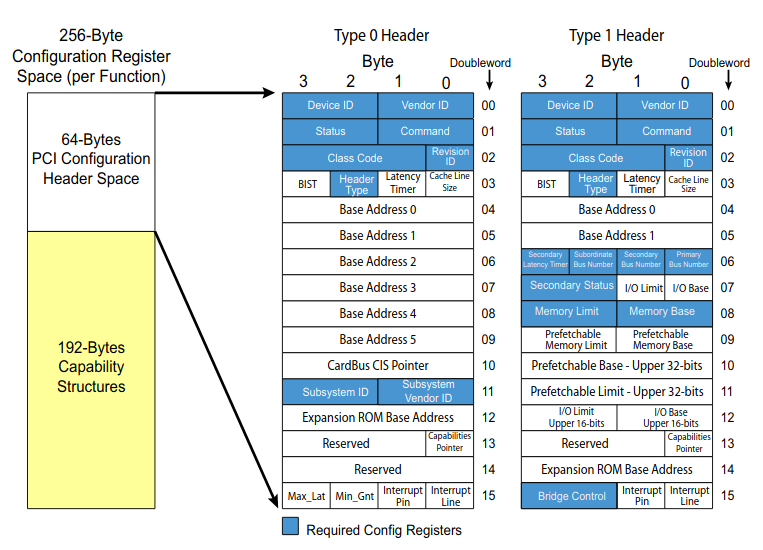
\includegraphics[width=\textwidth, keepaspectratio]{pics/pci-compatible-configuration-space.png}
  \caption{{PCI Compatible Configuration Register Space (Jackson, 2012, p.89)}\cite{book_pci_express}}
  \label{fig:pci-compatible-configuration-space}
\end{figure}

This section presents information on what the architecture and design of the solution look like. The next chapter explains how these design details apply to the implementation.


\chapter{Implementation}\label{Implementation}

The next part of the thesis provides implementation details. It presents key elements of the implementation and also what problems occurred in the development process. This completes all the theoretical and design information presented above.

Firecracker is a project that is implemented in Rust\cite{book_rust_programming}. Rust is a very strict programming language that brings more confidence to the developers. Pedantic compiler checks each variable one uses and every memory address reference. All its power comes from its ingenious type system that solves all those issues right at compile time. The very same design that prevents memory issues also prevents data races\footnotemark. Thus, the implementation of the PCI bus consists of creating a new crate within Firecracker. A crate is a compilation unit in Rust, meaning a binary or a library.
\footnotetext{\url{https://medium.com/paritytech/why-rust-846fd3320d3f}}

The first step of implementation was to build components of the PCI Express system. There are separate files for the PCIe bus, device, and function to maintain the modular structure and design of the project. Thereby, a function is a component where the configurations related to the devices exist. An array of 32-bit unsigned integers represents the configuration space of a function. The module contains methods to access this space and other specific constants and enumerations. The bus and the device structures represent wrappers around devices and functions. A bus contains a hash-table with all the devices that connect to it. A device contains two hash-tables, because, depending on its type, both other devices or other buses can connect to it. The header type decides this capability if the device is a general one or it is a switch/bridge. A general device is an endpoint, while other nodes can connect to a switch/bridge. So, this step involved the representation of the relationships between the components presented in figure~\ref{fig:pcie-topology}.

Further, the next stage consists of creating the initial device considering the existing code in the Firecracker project. The Host Bridge (part of the Root Complex), connects to the bus exposed by the Port-based I/O Manager. Connecting to this manager involves two requirements. The first one is that the Host Bridge structure must be encapsulated in the structure of the PIO manager. The second condition is that the new device has to implement certain imposed Rust traits. A trait is a collection of methods defined for an unknown type. For example, for the Host Bridge to be able to connect to the existing bus, it must implement a \textit{BusDevice} trait which contains \textit{read}, \textit{write}, and \textit{interrupt} methods. One should consider that this trait could change throughout the development of Firecracker project.

Thereby, the Host Bridge will intercept all reads and writes made in \texttt{CF8h-CFFh} address space. As already mentioned, there are two 32-bit registers in this space. At \texttt{CFCh} is a data register, so one will read data from it or will write data to it. The Configuration register only interprets information when the CPU makes a full 32-bit write to it. The information written to this space must have the template illustrated in figure~\ref{fig:configuration-CF8h}.

\begin{figure}[H]
\centering
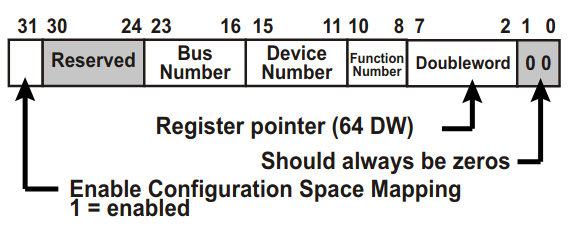
\includegraphics[width=\textwidth, keepaspectratio]{pics/configuration-CF8h.png}
  \caption{{Configuration Address Port at CF8h (Jackson, 2012, p.92)}\cite{book_pci_express}}
  \label{fig:configuration-CF8h}
\end{figure}

The bus number, device number, and function number will identify the target of the operation. The register pointer chooses the double word in the target configuration space. Because this register has only 6 bits length, it can select only one of the first 64 double words (so only PCI-compatible). The Root Complex node implements methods to decode this information. Further, it sends the requested operation to the specified target.

To make the synchronization between the address and data possible, RC (Root Complex) behaves like a state machine. Thus, when writing to the configuration address space, RC stores the value in one of its fields. At the next operation with the data register, the read/write operation will use the stored configuration address.

For the most part, the implementation consists of the device which represents the entry-point in the PCIe topology. Further, each entity has read/write methods that will validate the moving data. In the end, a device can be configured according to one of the layouts shown in figure~\ref{fig:pci-compatible-configuration-space}.

This implementation always developed taking into account the values of the Firecracker project. Each of the modules created has unit-testing. Individual units of source code are tested to determine whether they are fit for use. The application is robust even in a multi-threading environment. The Arc-Mutex mechanism of Rust protects against race conditions when accessing the PCI devices.  Thus, it is efficient, simplistic, and scalable. The written code is well documented and ready to be taken over without much effort by other developers.

This chapter presents the exact details by which the operating system of a microVM communicates with PCI devices. When starting a system, there is a process of enumeration of all connected PCI devices and initializing them. This process is also named PCI probing and it will represent the central point of the next chapter, the implementation evaluation.

\chapter{Evaluation}\label{Evaluation}

This section presents the evaluation of the results obtained by the work of this diploma project.

To assess the relevance and importance of the project I would like to note a few things. When I started the project, I announced my intention to the community, and since then, I have found answers and advice to all my questions. Moreover, developers from other projects reached out. They highlighted the importance of this diploma project work for them. Thus, people who use Firecracker made their help available to me, in case I needed it.  One such example is the community around the Weaveworks project\footnote{\url{https://www.weave.works}}. Weaveworks Ignite\footnote{\url{https://www.weave.works/blog/fire-up-your-vms-with-weave-ignite}} is an open-source VM with a UX container and built-in GitOps management. It is fast and secure because it combines Firecracker MicroVMs with Docker/OCI images to unify containers and VMs.

The implementation of the required functionality can be verified by logs and Linux commands. Thereby, to be able to evaluate and validate the existence of a PCI bus in a Firecracker microVM, one can perform the following steps:
\begin{itemize}
    \item get the Firecracker source code\footnote{\url{https://github.com/firecracker-microvm/firecracker}} which contains the implementation of the PCI bus.
    At the time of writing, the implementation has not been verified due to the busy schedule of maintainers. It can be found in the author personal repository\footnote{\url{https://github.com/andreiraduta1101/firecracker/tree/feature-pci}}.

    \item follow the instructions from the Firecracker documentation to create a new instance using custom kernel and rootfs images. An important thing here is that the kernel image will need to have PCI/PCIe support enabled.

    \item the current directory should contain:
    \begin{itemize}
        \item Firecracker binary.
        \item rootfs image.
        \item kernel decompressed image.
        \item JSON file with the guest virtual machine configuration.
    \end{itemize}

    \item start the Linux instance using the instructions from documentation.
\end{itemize}

The Rust code configures the connected Host Bridge. Its Vendor ID is \texttt{1D94h} and its Device ID is  \texttt{1452h}.  The listing~\ref{lst:pci-check} depicts the commands that will start a microVM and check the PCI existence. The \texttt{dmesg} (diagnostic message) command prints the message from the kernel, so, from the operating system. It will show all the information about the PCI bus if it is present, including initialization errors.

\lstinputlisting[caption={PCI Check}, label={lst:pci-check}]{pci-check.sh}

First, the operating system allocates special memory space for the PCI devices. The size of this space is 768 MB. Here is the area where the devices will receive the required memory.

According to the \texttt{lspci} command manual\footnote{\url{https://linux.die.net/man/8/lspci}}, the meaning of the values on the last line is:
\begin{itemize}
    \item \texttt{00:00.0} - bus 0, device 0, function 0.
    \item \texttt{Class0600} - PCIe Device Class for Bridge Devices\footnote{\url{https://pci-ids.ucw.cz/read/PD}}.
    \item \texttt{1d94:1452} - PCIe Dummy Host Bridge Vendor ID and Device ID\footnote{\url{https://devicehunt.com/view/type/pci/vendor/1D94/device/1452}}.
    \item \texttt{0000:0000} - System Vendor (optional) and System Device (optional).
\end{itemize}

Second, during PCI enumeration (PCI hardware probing), one can see that there is only one discovered and connected device. That is the dummy configured device and it takes the role of Host Bridge. The \texttt{lspci} command confirms the previous statement.

For even more detailed verification of the correctness of the implementation, tests are available:
\begin{lstlisting}[caption={Testing}]
# PCI unit tests.
andreir@X750LN:~/firecracker/src/pci/src$ cargo test

# Firecracker integration tests.
andreir@X750LN:~/firecracker$ tools/devtool test
\end{lstlisting}


\chapter{Conclusions and Further Work}\label{Conclusions and Further Work}

Firecracker is a real innovation that combines the notions of virtual machines and containers. What makes it so powerful is its simplicity and adaptability. Its team of developers adds new features to this project both according to the requirements of the customers and the open-source community.

Currently, a PCI/PCIe bus is present in both personal computers and high-performance systems. Also, this component is becoming a key point in virtualization. It can lead to lower downtime through hot plugging and improved performance by providing a way to achieve passthrough devices virtualization.

The goal and the outcome of this diploma project are to combine these two mentioned aspects. Emulating a PCI bus in each virtual machine created by Firecracker improves its present performances and creates new usages. At the same time, this makes this hypervisor a very good solution for a multitude of projects in which virtualization is a necessary aspect.

The implementation consists of connecting the Root Complex node of a PCIe topology to the Firecracker. So, the Host Bridge piece of Root Complex will connect to the PIO (Port-based I/O) device manager. The Host Bridge will interpret all read/write operations that the Operating System performs in the I/O memory space intended for PCI. This means that it will communicate on behalf of the CPU with the connected devices through the PCI bus.

Next, further developments will focus on creating a device that works using the PCI bus. A clone of an already functional device (for example, the networking device) is a valid starting point. The clone will receive the necessary changes to communicate with the system via the PCI protocol. Thus, having two almost identical devices, the performance difference is easy to measure with before/after tests. Also, a new device that performs the same functionalities can be built from scratch, taking advantage of the new architecture.

Another point that opens the way for a lot of improvements is the interrupt system. PCI defines (MSI) message signaled interrupts. These are an in-band alternative to replace traditional out-of-band interrupt lines. This method uses special messages to announce that a device triggers an interrupt. MSI allows the device to write a small amount of data to a special memory address that describes the asserted interrupt. In other words, pin assertion and de-assertion are emulated. The first advantage is the increase in the possible interrupts numbers. The second advantage is performance improvement. This happens because when using legacy interrupts, memory writes have to be double-checked to avoid possible race conditions. Putting in place this functionality requires a more advanced interrupt manager, and Firecracker does have it.

\bibliographystyle{plain}
\bibliography{bibliography}\addcontentsline{toc}{chapter}{Bibliography}

\end{document}
